\documentclass[10pt]{article}
\usepackage[margin=2.4cm]{geometry}
\usepackage{graphicx}
\usepackage{booktabs}
\usepackage{xcolor}
\usepackage[hidelinks]{hyperref}
\usepackage{parskip}
\definecolor{jblue}{HTML}{2A78D6}
\definecolor{jrand}{HTML}{EB6834}
\definecolor{jnonj}{HTML}{1BAF7A}
\definecolor{jlogitdict}{HTML}{8A5CF5}
\newcommand{\code}[1]{\texttt{\small #1}}

\title{\textbf{J-space, Part 2: The Model Matrix}\\
\large From lab result to publishable finding --- living handout}
\author{karlb-dev\thanks{Draft campaign handout; grows a subsection per
banked phase. Part-1 handout: \code{jspace/handout/olmo32b\_jspace\_handout.pdf}.}}
\date{Campaign started 2026-07-27 --- preregistered before data (\code{27c6d3c})}

\begin{document}
\maketitle

\section{Where Part 1 left off, and what Part 2 must decide}

Part 1 (Lab 37) replicated the descriptive geometry of the Anthropic
workspace paper on \code{Olmo-3-32B-Think} at $\sim$10$\times$ thinner
capacity, found the paper's static causal dissociation \emph{null} on both
OLMo and \code{Qwen3.6-27B} under energy-matched instruments, established
per-item frozen J-ablation as a control-clean cross-model causal handle on
retrieved content ($-2.9$/$-2.4$ nats), and measured a foil-calibrated
46-step workspace-ahead-of-text lead. Part 2 adjudicates \emph{why the
dissociation is missing}:

\begin{center}\small
\begin{tabular}{llp{7.6cm}}
\toprule
 & hypothesis & discriminator \\
\midrule
H1 & externalization (think-training moved the workspace into tokens) &
Workstream A: matched-pretraining sibling \code{Olmo-3.1-32B-Instruct},
Qwen matrix completion, \code{gemma-4-31B-it} \\
H2 & occupancy (live J-space $\approx$ the output stream itself) &
Workstream D: output-occupancy index across the matrix \\
H3 & training-lab specifics & unfalsifiable; shrunk by exhausting the rest \\
H5 & residual instruments & B (frozen-logit, fit-size, Dolma corpus,
dose/persistence selection), C (load-demanding tasks, paper's own sets) \\
\bottomrule
\end{tabular}
\end{center}

Standards: $n\ge60$ headline cells, two seeds on decisive grids, bootstrap
CIs, BH-FDR across the matrix, preregistered directional predictions
(\code{preregistration.md}).

\section{Workstream A}

\subsection{A0 --- does the J-dictionary survive post-training?}

The part-1 Think lens, applied unchanged (donor $J$, recipient unembedding)
to \code{Olmo-3.1-32B-Instruct} --- same base model, different
post-training. Preregistered gate: probes $\ge$15/21 and multihop pass@1
$\ge 0.85\times$ donor $=0.2408$.

\begin{figure}[h]
\centering
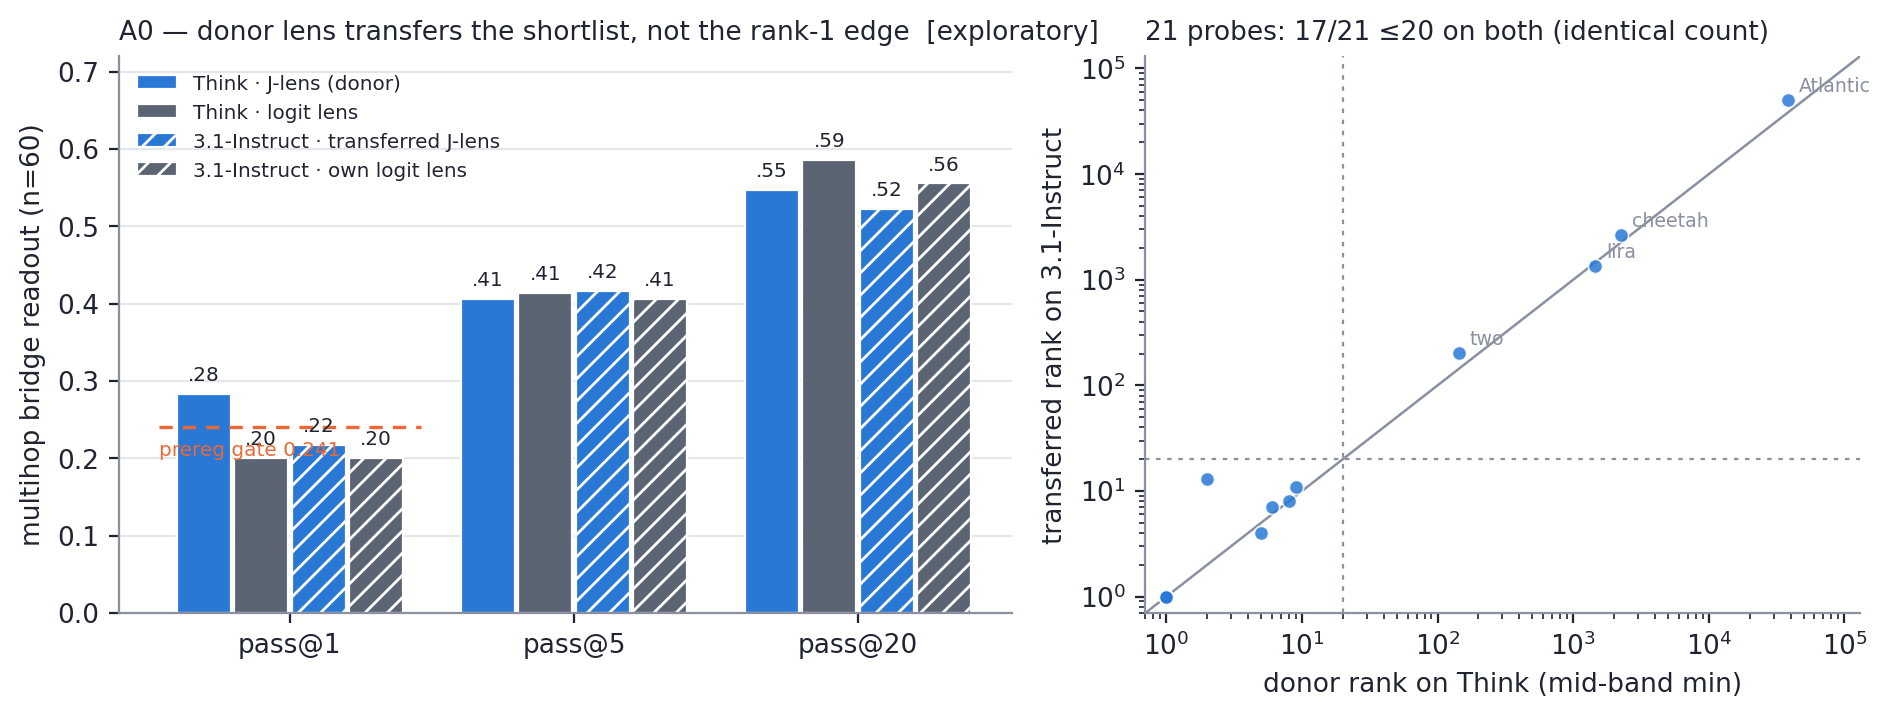
\includegraphics[width=\linewidth]{figures/p2f1_a0_transfer.png}
\caption{\textbf{A0 transfer gate.} Left: the transferred lens reads the
bridge-entity \emph{shortlist} at donor level (pass@5 0.417, pass@20 0.522
vs donor 0.41/0.55) but loses the rank-1 edge (0.217 vs 0.283, below the
preregistered floor, dashed). Right: per-probe mid-band ranks --- 17/21
$\le$20 on \emph{both} models, same items missing.}
\end{figure}

\textbf{Verdict: \code{TRANSFER\_FAIL}, informative.} The readout basis is
static across post-training (unembed row cosine median $0.9984$; final-norm
gain cosine $1.000$), direct-fact probes transfer exactly (17/21 both), the
shortlist transfers --- what post-training blunted is specifically the
\emph{rank-1 sharpening}, the very component that was the J-lens's
distinctive advantage on Think ($+41\%$ relative pass@1 there, $+8.5\%$
here). The prereg FAIL rule fires: fit the sibling's own 120-prompt lens.
Recovery to $\sim$0.28 $\Rightarrow$ mid-band J-map drift under
post-training; no recovery $\Rightarrow$ Instruct resolves the silent
bridge more weakly --- itself an H1-flavored datum.

% \subsection{A1 --- Core Battery on Olmo-3.1-32B-Instruct} (pending)

\section{Workstream B}

\subsection{B3 --- does the causal handle need the Jacobian? [exploratory pilot]}

\begin{figure}[h]
\centering
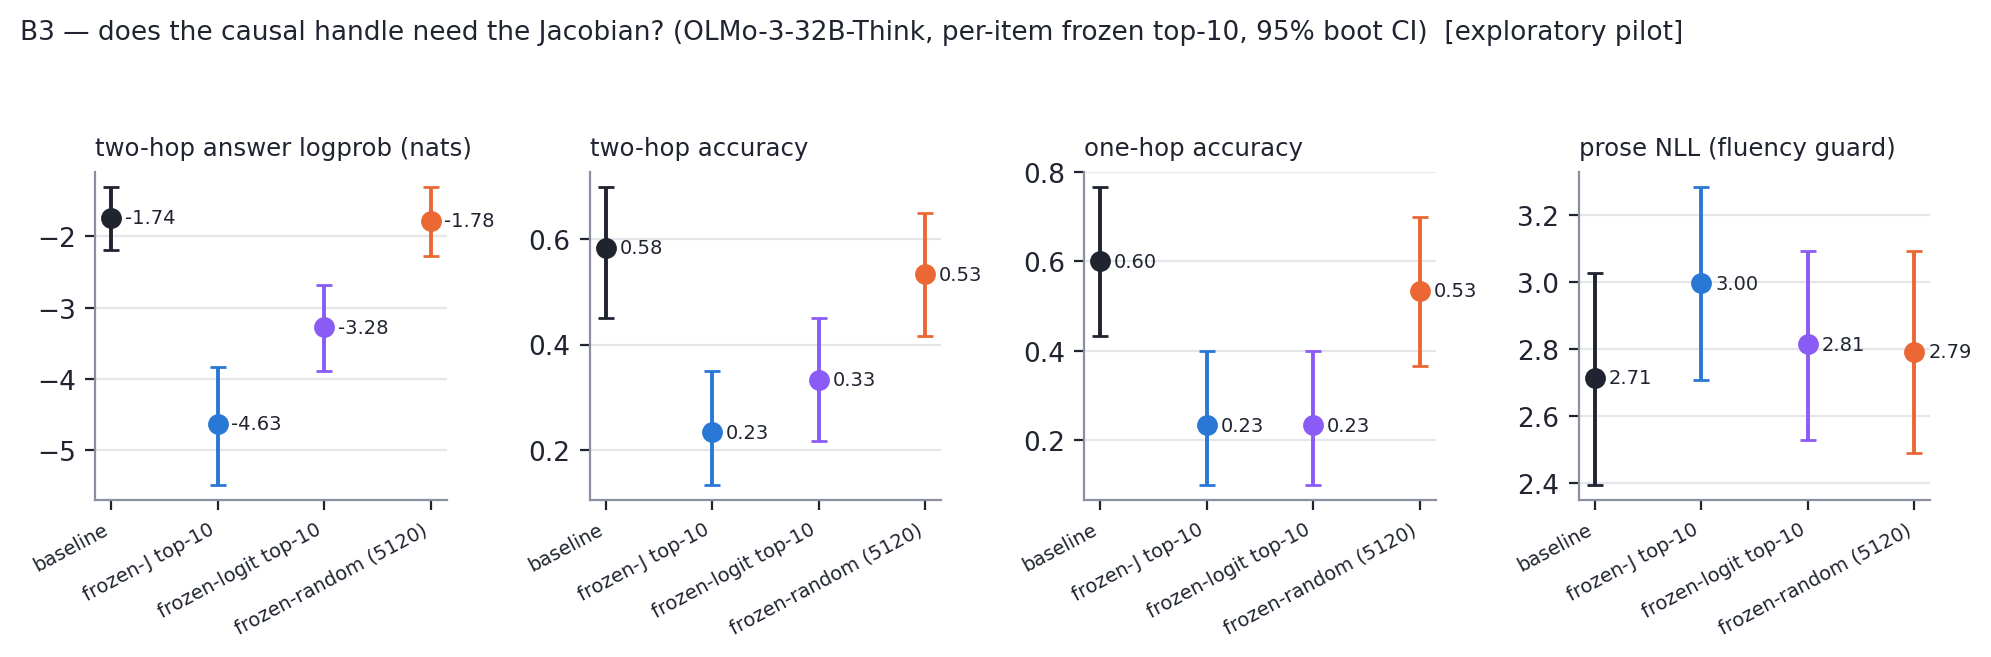
\includegraphics[width=.92\linewidth]{figures/p2f2_b3_frozen_logit.png}
\caption{\textbf{B3.} The frozen-\emph{logit} dictionary (no Jacobian,
violet) reproduces $\sim$53\% of frozen-J's two-hop logprob deletion
($-1.54$ vs $-2.90$ nats) and the \emph{identical} one-hop collapse
(0.23=0.23), while the random twin sits on baseline. Output-aligned
directions alone carry much of the part-1 marquee effect; the geometry
control family (R3) adjudicates the rest.}
\end{figure}

\section{Workstream R --- assay repair (the addendum's mandate)}

\subsection{R7 pilot --- the paper's output-protected ablation, run faithfully}

\begin{figure}[h]
\centering
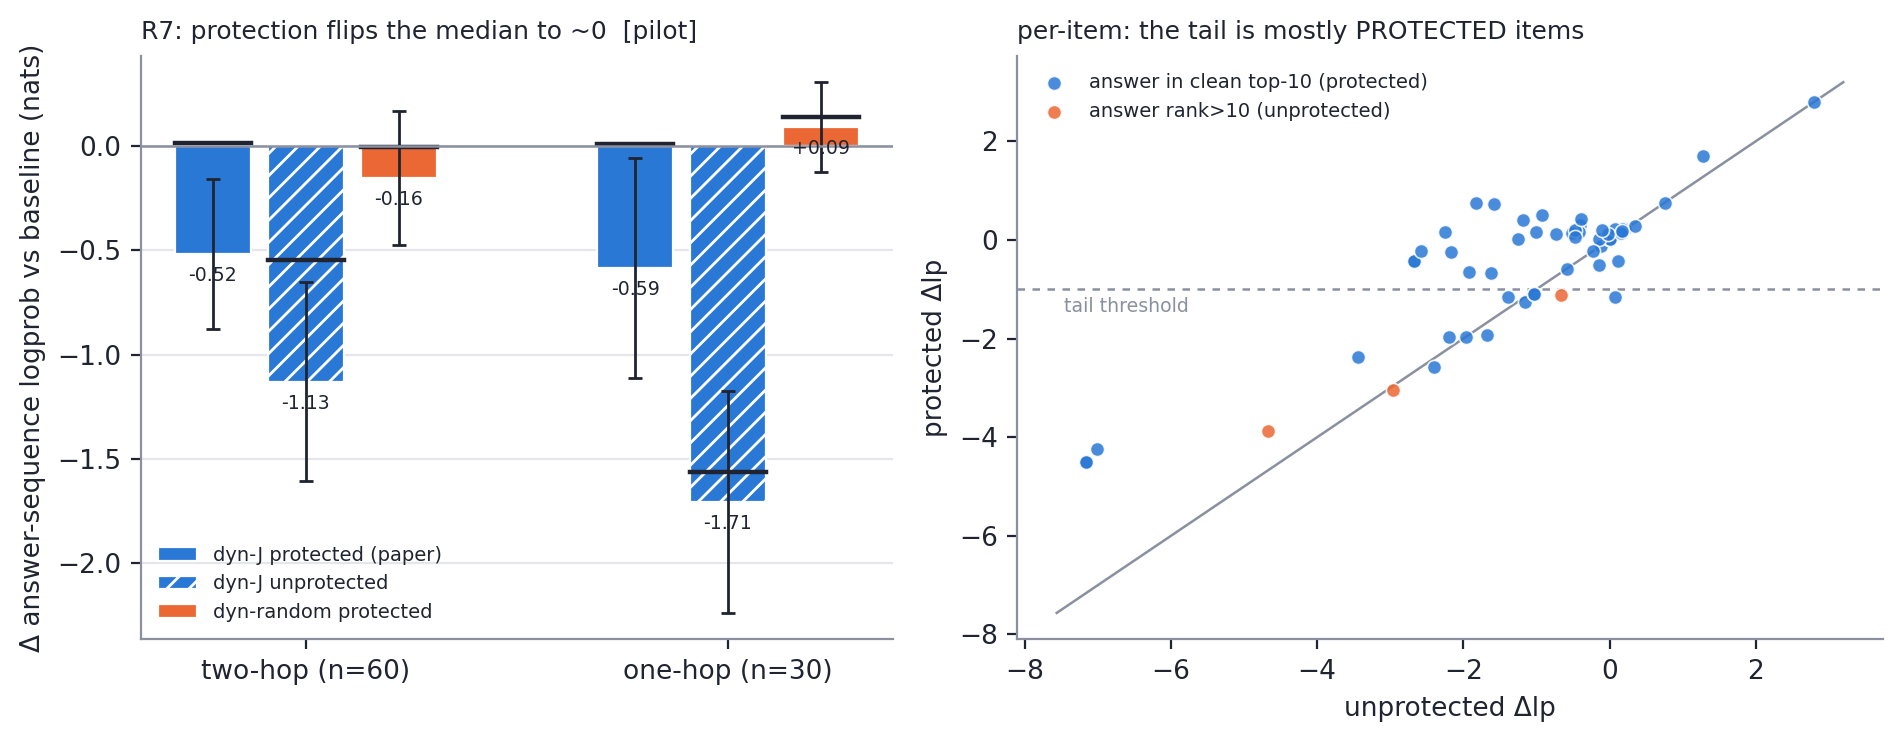
\includegraphics[width=\linewidth]{figures/p2f3_r7_protected.png}
\caption{\textbf{R7 pilot (Think).} Left: with the paper's clean-output
top-10 protection, the \emph{median} item is untouched (two-hop $+0.02$,
one-hop $+0.01$ nats) while the unprotected twin deletes hard
($-0.55$/$-1.56$ median) --- part-1's live-ablation damage was mostly
output-stream deletion (H2, causal form). Right: a J-specific tail
survives protection (16/60 two-hop items lose $>1$ nat; protected-random
on the same items: $+0.34$), and 13 of those 16 have the answer at clean
rank 1--3 --- \emph{explicitly protected yet still deleted}: indirect
J-content damage (bridge-entity reading), the confirmatory grid's prime
target.}
\end{figure}

\subsection{R2 --- capacity under the paper's own estimator}

\begin{figure}[h]
\centering

\includegraphics[width=.92\linewidth]{figures/p2f4_r2_occupancy.png}
\caption{\textbf{R2 pilot.} Marginal-gain occupancy (frozen crossing
rule, 3 random control dictionaries) and excess variance share at median
occupancy. Both OLMo siblings: occupancy median 2, excess $\le 0.9\%$ ---
far below the paper's Claude band (10--25, 6--10\%), identical across the
post-training pair. The Qwen recompute under this same estimator is the
decisive cross-model capacity cell.}
\end{figure}

\subsection{R7 cross-model + R2-Qwen --- the campaign headline (pilot)}

\begin{figure}[h]
\centering
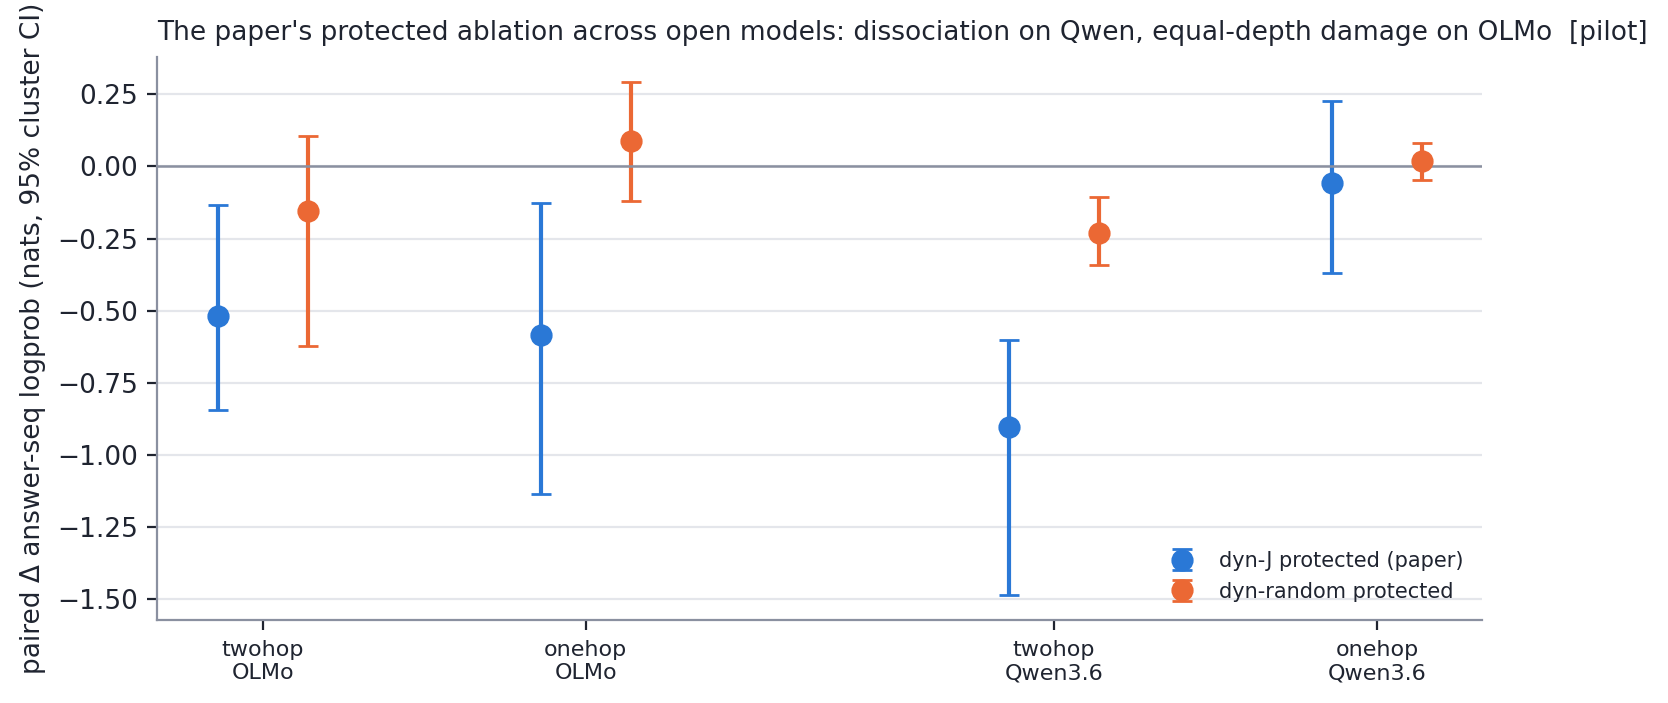
\includegraphics[width=.9\linewidth]{figures/p2f5_crossmodel_protected.png}
\caption{\textbf{Capacity and causal signature co-vary.} Under the
identical protected protocol (paired family-clustered CIs): Qwen3.6-27B
shows the paper's dissociation shape --- two-hop $-0.91$
$[-1.49,-0.60]$, one-hop $-0.06$ [straddles 0] --- while OLMo-3-32B-Think
shows equal-depth content damage ($-0.52$/$-0.59$, both excl.\ 0, plus
the indirect protected tail). The same models order the same way on
paper-defined occupancy (3--4 vs 2, excess 1.0--2.2\% vs
$\le$0.9\%), and BOTH sit an order of magnitude below the paper's Claude
band (10--25, 6--10\%) --- with lens fit size ruled out (Qwen used the
published $n{=}1000$ lens). Lens robustness: two independent 120-prompt
Instruct fits agree at dictionary row-cos 0.993 and frozen-selection
Jaccard 0.806.}
\end{figure}

\subsection{The four-model ladder --- the causal signature reorganizes}

\begin{figure}[h]
\centering
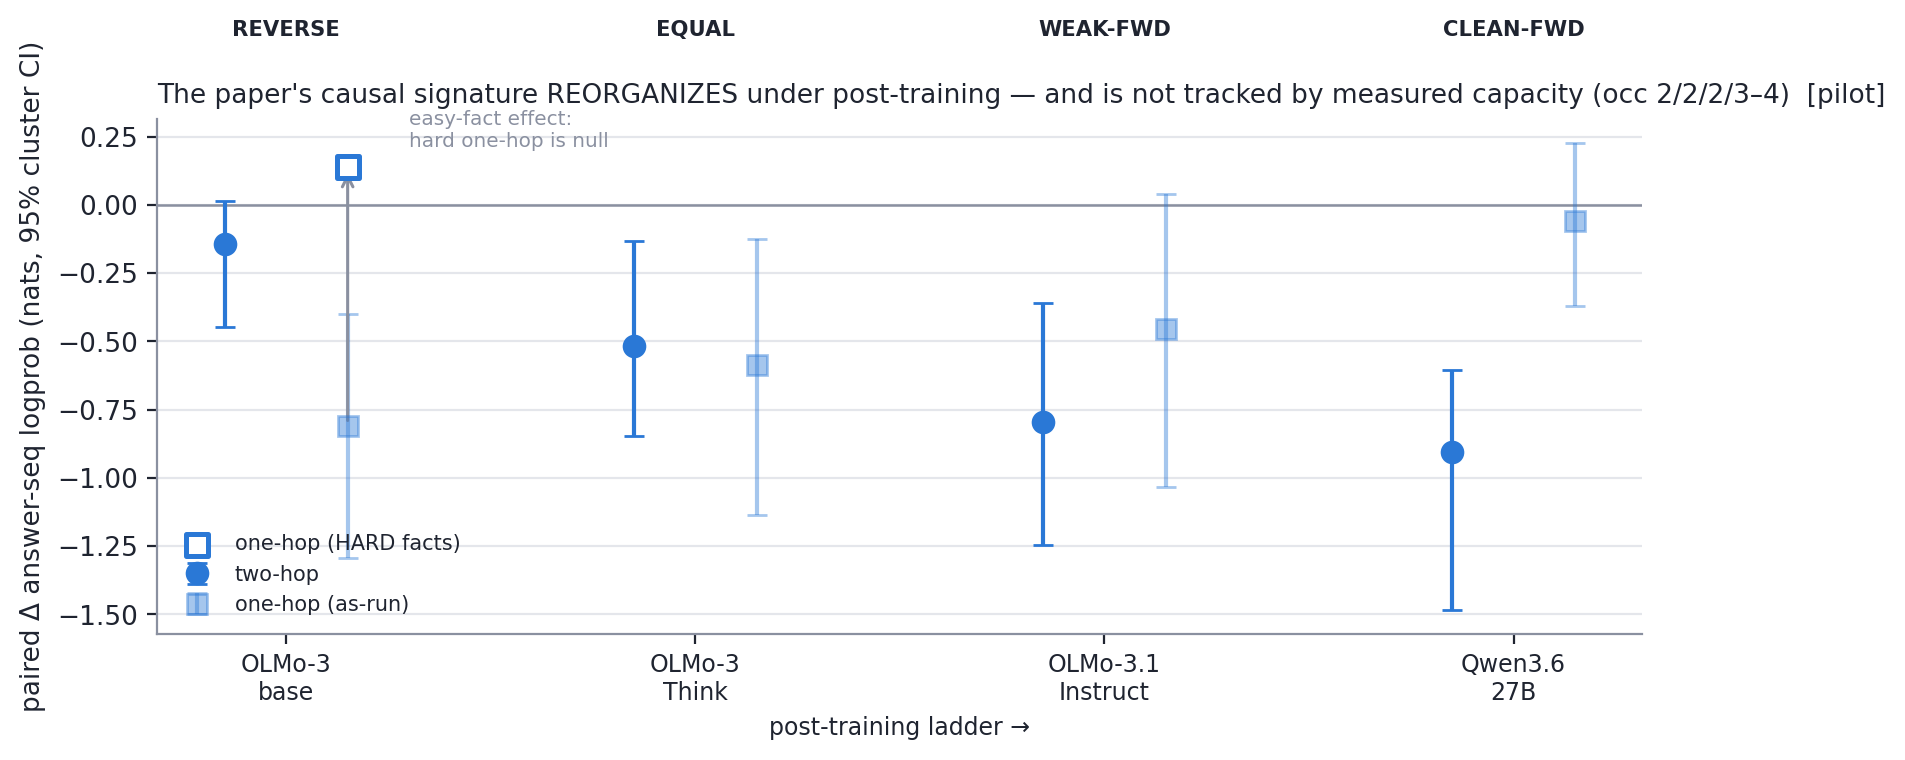
\includegraphics[width=.95\linewidth]{figures/p2f7_ladder.png}
\caption{\textbf{The paper's causal signature is not a fixed property of
``an LLM'' --- it reorganizes along post-training.} Protected dynamic
J-ablation, paired family-clustered CIs, four checkpoints: the base model
shows a REVERSE dissociation (one-hop hit, two-hop spared), Think shows
equal-depth damage, 3.1-Instruct a weak forward dissociation, Qwen the
paper's clean shape. Measured capacity does \emph{not} track this
(occupancy 2/2/2/3--4): Instruct and Think are identical on capacity and
differ on shape. The open marker records the ceiling check that relabeled
the bottom rung --- on \emph{hard} one-hop facts the base effect is null
($+0.14$; matched random $-0.01$), so the $-0.81$ was an EASY-FACT
effect: rehearsed facts occupy the deletable output-adjacent channel and
hard facts do not. Confirmatory hypotheses are therefore stated in
fact-accessibility terms, not task depth.}
\end{figure}

\subsection{What the protected ablation actually deletes (tail mechanism)}

The selected-id instrument logs, per layer and position, which dictionary
rows the ablator deflates. On Olmo-3-32B-Think: the two-hop bridge
entity's tokens are deflated on \textbf{95\%} of items versus
\textbf{2\%} under a bridge-reassignment permutation
($p<0.0005$) --- the J-directions really do carry the intermediate
entity. But this is \emph{universal}: 0.94 on the damaged tail versus
0.95 on undamaged items, so bridge deletion alone is not sufficient for
damage. What separates the tail is (i) protection failure --- 21\% of
tail items had answers outside the protected clean-top-10 versus 0\% of
non-tail --- and (ii) among the 19 tail items whose answer \emph{was}
protected, lower model confidence (median clean rank 2 versus 1).
Deleting workspace content costs the model only when the answer is not
already locked in.

\subsection{Gemma-4-31B: an architecture datum with a depth}

\begin{figure}[h]
\centering
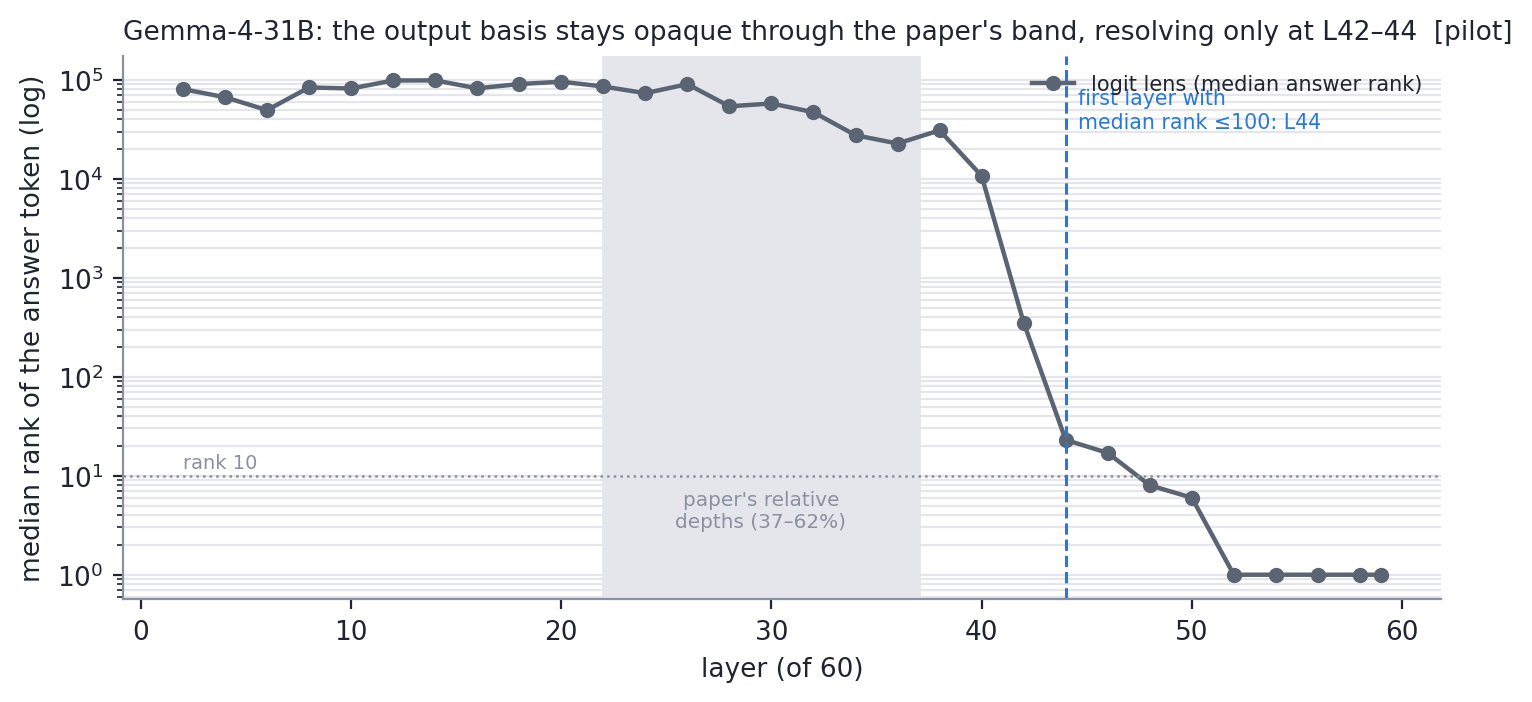
\includegraphics[width=.92\linewidth]{figures/p2f8_gemma_depth.png}
\caption{\textbf{Gemma's residual stream is opaque in the output basis
through exactly the band the paper studies.} Median rank of the answer
token by layer, read with the reference unembedding (final norm, tied
head, softcap~30). Ranks stay in the tens of thousands from L2 to L40 and
collapse abruptly at L42--44, reaching rank~1 by L52. The paper's
relative depths (37--62\%, i.e.\ L22--L37) sit entirely inside the opaque
zone. The vanilla logit lens and the Jacobian micro-lens fail
\emph{equally} here, so this is a property of the model family, not of
the instrument. Whether Jacobian transport rescues mid-band readability
is the question the full 120-prompt fit answers; no family verdict is
stated until it lands.}
\end{figure}

\subsection{Design consequence: the confirmatory endpoint must change}

The G6 power simulation, calibrated on the pilot parquets, finds that
protected paired deltas are a zero-mode plus heavy-tail mixture. The
drafted 0.5-nat \emph{mean} primaries are structurally underpowered. This
subsection's original ICC figure ($\approx0.40$, apparently uniform across
models) is \textbf{superseded} --- see \S\ref{sec:vm8}.

\section{VM8 --- the repair block that changed the design}\label{sec:vm8}

A second forensic review was accepted and executed. Four repairs moved
numbers that appear earlier in this handout; where they disagree, this
section wins.

\subsection{The clustering unit was wrong, and it was load-bearing}

Every family-clustered interval, ICC and the power simulation above used
\code{name.split("-")[0]} as the statistical family. That is a string
accident: \code{atomic-80-state} and \code{ex-element-state-80-8} are the
same template but landed in different families, sixteen unrelated items
shared the family \code{ex} because their names begin with those letters,
and each of the ten one-hop ``capital of X'' items was its own family.
Under a hand-audited map (120 items, rule \emph{(second-hop relation,
answer type)}) the pilot's 60 two-hop items are \textbf{25 canonical
families, not 38 raw labels}, one of which holds 11 of the 60.

Point estimates are unchanged --- clustering touches uncertainty, not
means. What moved is the apparent homogeneity: audited ICC is 0.66
(base), 0.56 (Think), 0.17 (Instruct), 0.75 (Qwen), against a uniform
0.37--0.42 before. \textbf{One conclusion flips}: Instruct's one-hop
interval moves from $-0.45\,[-1.03,+0.06]$ to $-0.45\,[-1.29,-0.01]$, so
the ``weak forward dissociation'' rung of the four-model ladder is
withdrawn --- it reads as equal-depth damage. It is knife-edge and
reverses again under family weighting, which is why the preregistration
candidate fixes the weighting estimand in advance.

\begin{figure}[h]\centering
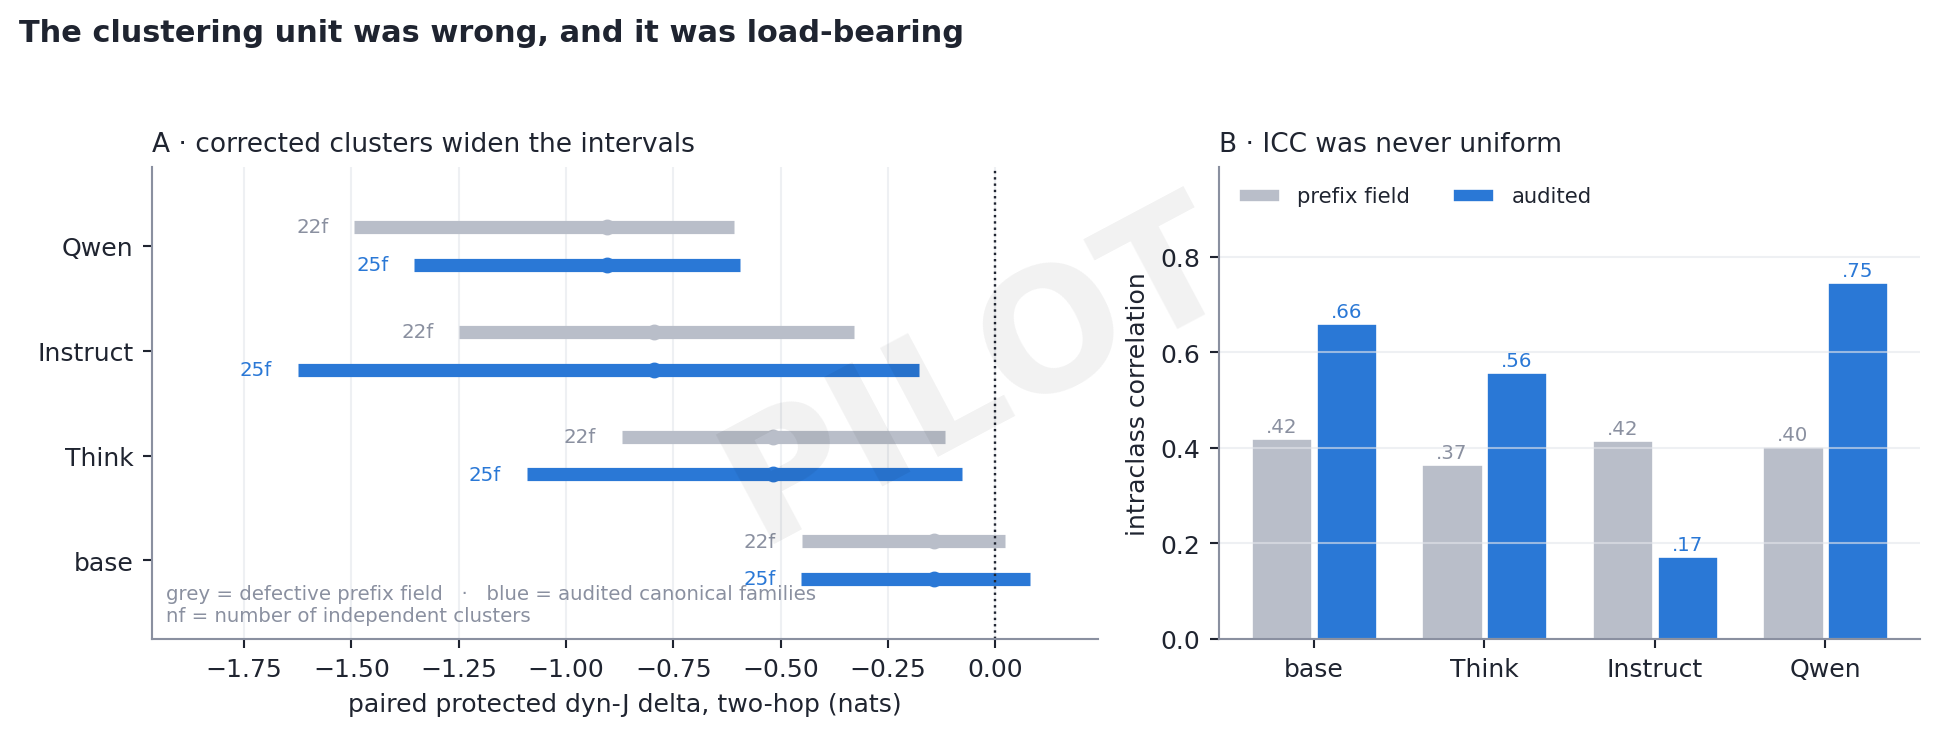
\includegraphics[width=\linewidth]{figures/p2f10_family_correction.png}
\end{figure}

\subsection{At 60 families, only two cells can carry a binary test}

Inverting the power question --- given $m$ families, what is the smallest
detectable effect at 90\%? --- gives, at the 60 canonical families the
bank now holds: OLMo Think needs a 0.30 rate difference to see its 0.133
pilot gap ($2.3\times$ short), Instruct 0.30 against 0.100
($3.0\times$ short). Only \textbf{Qwen on the rate endpoint} and
\textbf{Instruct on the mean endpoint} are testable, and the two
endpoints have \emph{opposite} feasibility profiles across models. The
candidate therefore states most hypotheses as estimation with intervals
and declares a test only where power exists.

\begin{figure}[h]\centering
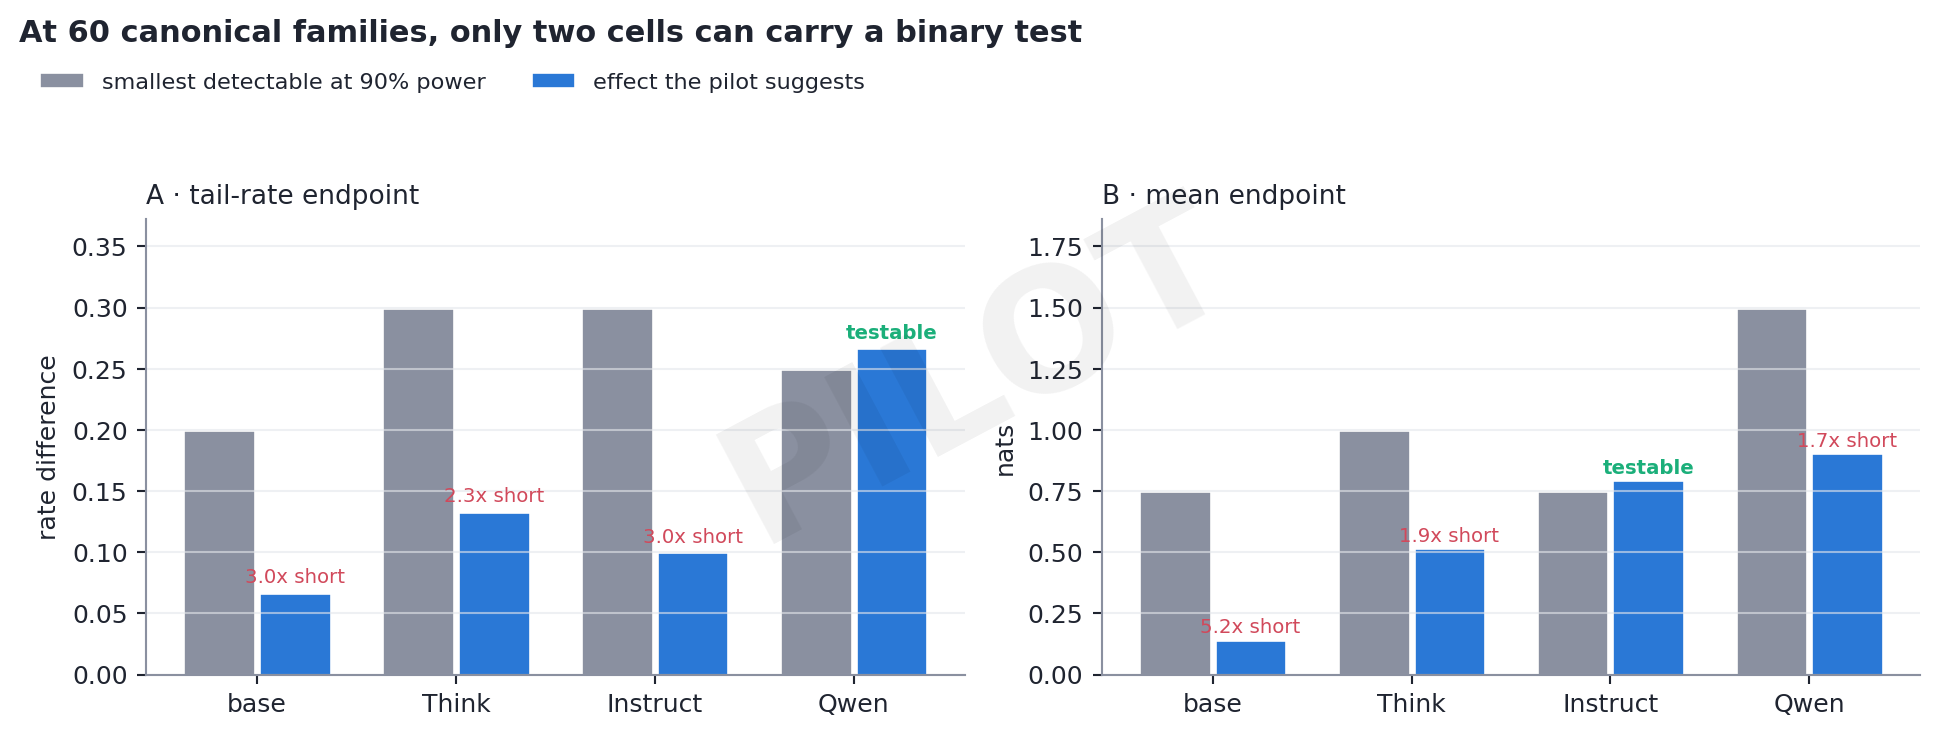
\includegraphics[width=\linewidth]{figures/p2f11_feasibility.png}
\end{figure}

\subsection{The averaged Jacobian's in-band gap is a ceiling}

For a \emph{uniform} perturbation the per-position and corpus-averaged
estimators are algebraically identical, $\sum_s J_s d = P (\overline{J}) d$,
so the earlier faithfulness test could not see position-averaging loss at
all. Perturbing one position at a time --- what the dynamic ablation
does --- separates them. Position-conditioning does \textbf{not} improve
response direction at any band layer ($-0.05$, $-0.04$, $-0.02$), though
it roughly halves the magnitude error. Cell by cell, cosine tracks the
ground truth's \emph{own} local linearity at within-layer Pearson
$r=0.76$--$0.90$ ($n=144$): the estimator is not the binding constraint.
Along the lens's own top rows --- where the ablation acts --- in-band
cosine is \textbf{0.58} versus \textbf{0.33} for random probes, so the
often-quoted ``$\sim$0.2 in band'' overstates the problem for the actual
intervention. The context-J methods arm fails its committed dev gate and
is not admitted.

\begin{figure}[h]\centering
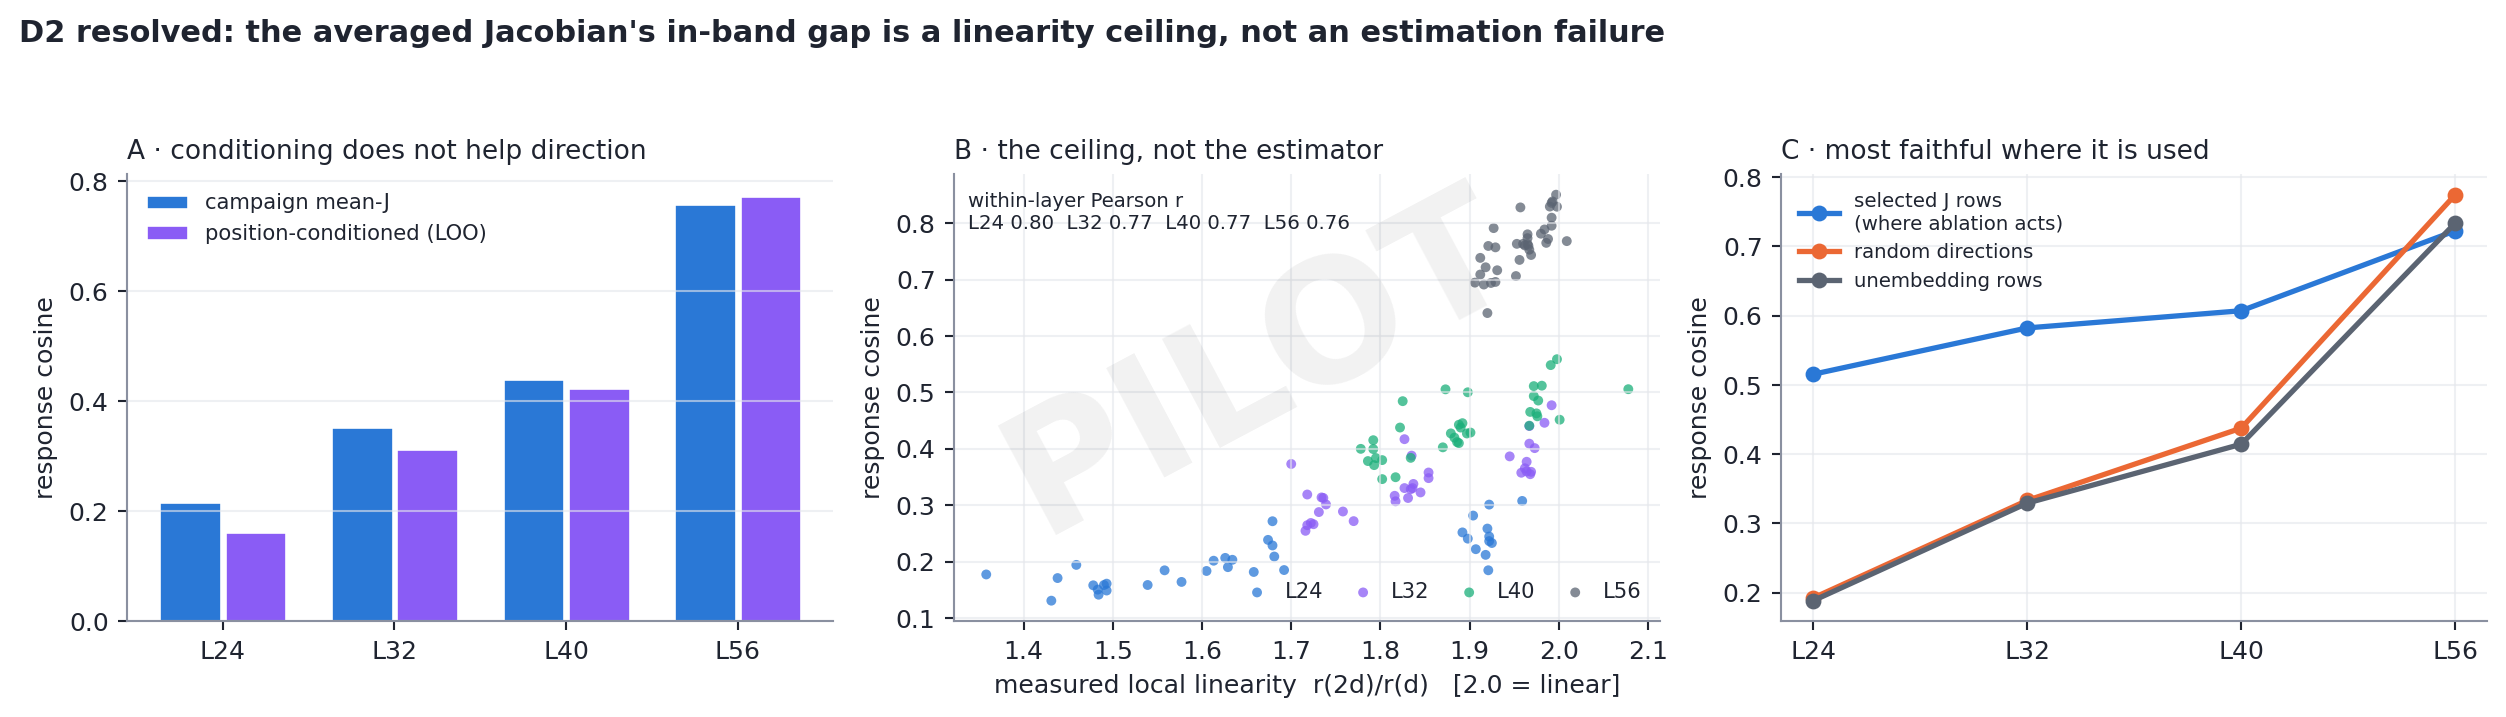
\includegraphics[width=\linewidth]{figures/p2f12_h7_ceiling.png}
\end{figure}

\subsection{Capacity: mislabelled, corrected, and still an order of magnitude low}

The v1 estimator computed a centered activation and never used it; both
shares were raw energy while the prose called them centered excess
variance. Occupancy is unchanged (median 2 --- it never depended on the
share definition). Centered $R^2$ excess is 0.49/1.02/\textbf{1.27\%}
against raw 0.03/0.54/0.80\%. The headline survives in slightly stronger
form.

\begin{figure}[h]\centering
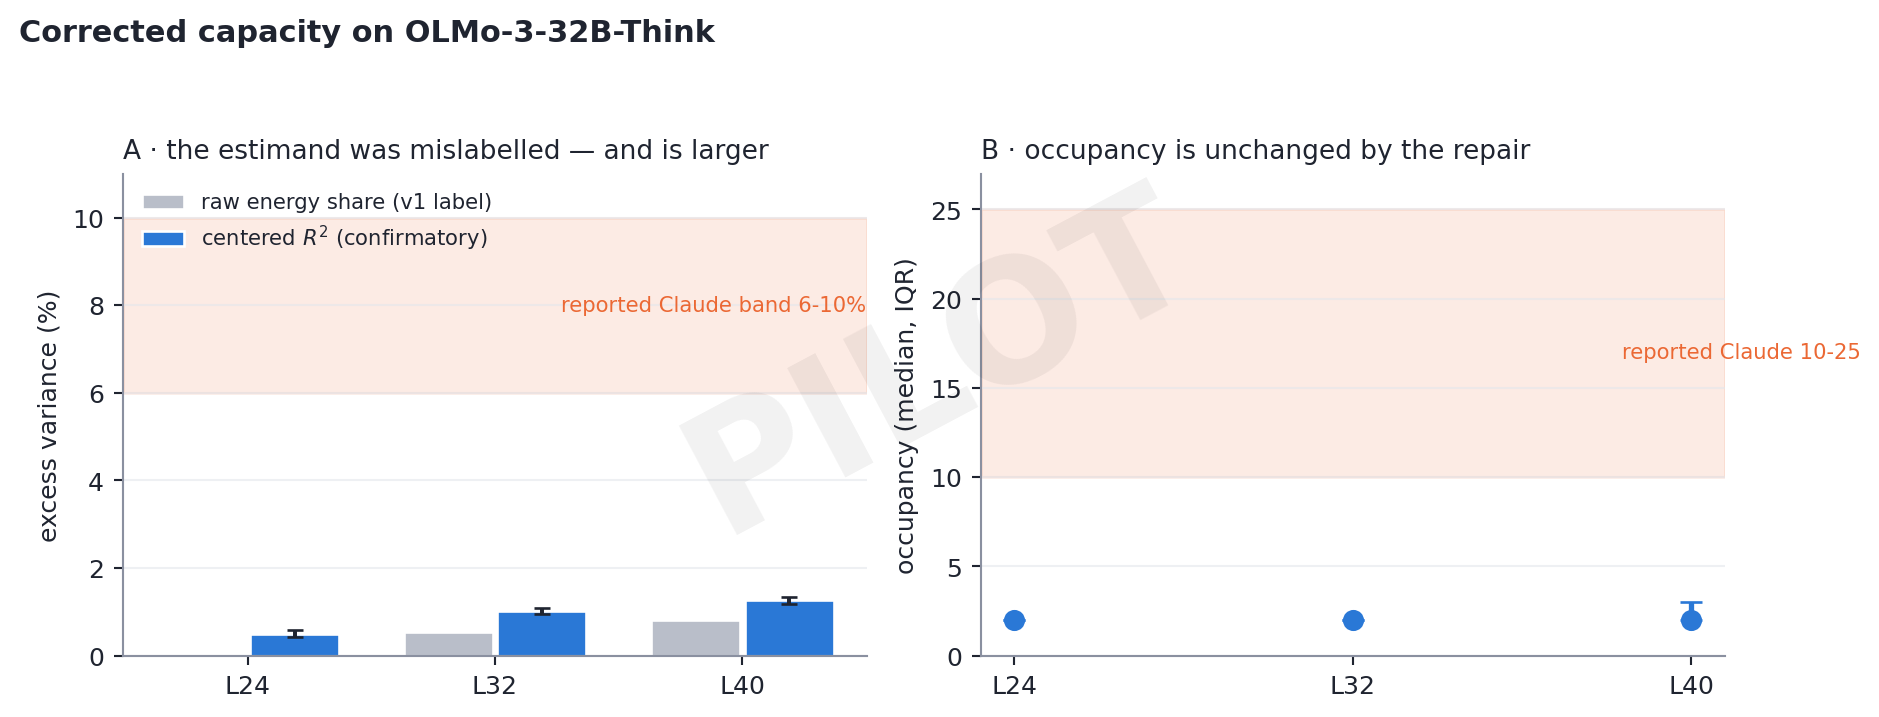
\includegraphics[width=.92\linewidth]{figures/p2f13_capacity_corrected.png}
\end{figure}

\subsection{G5 passes, and catches the author}

The task gate was run rather than waived. 1052 items, 15 excluded for
answer-in-prompt leakage, zero bridge leakage, every two-hop item
carrying its swap counterfactual, and \textbf{64 canonical families with
$\geq$3 capable items} against a target of 60. The duplicate-fact audit
caught nine newly authored ``families'' that re-expressed existing
relations, four of them sharing literal facts --- which would have let one
fact land in both the confirmatory and the replication partition.

\begin{figure}[h]\centering
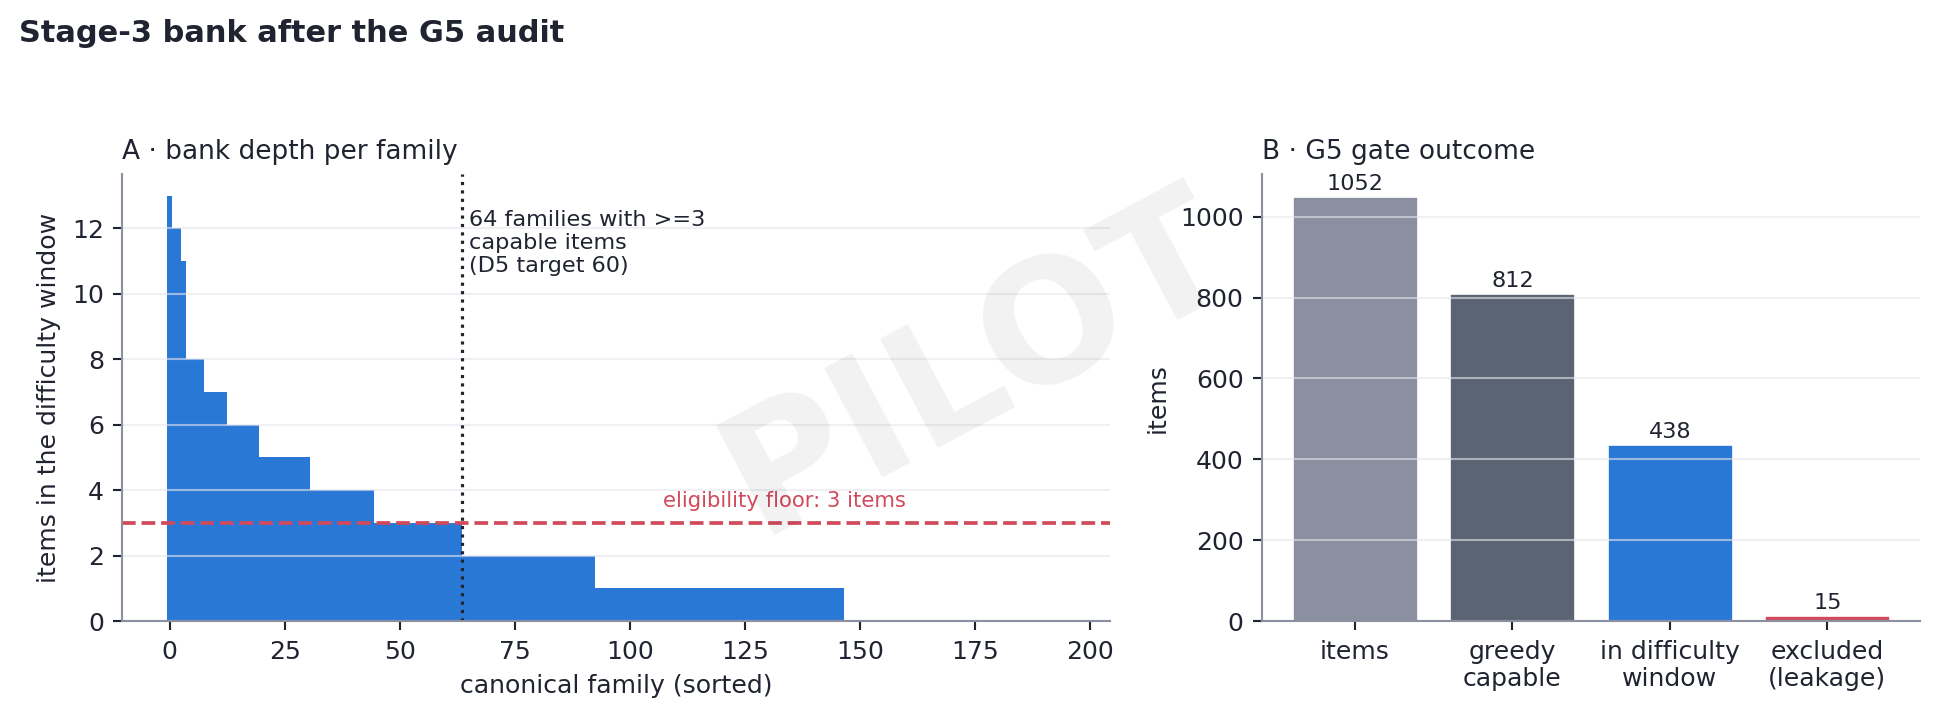
\includegraphics[width=\linewidth]{figures/p2f14_bank_readiness.png}
\end{figure}

\subsection{Status}

The preregistration \textsc{candidate} is written and the campaign is
\textbf{stopped at the freeze boundary} awaiting principal-investigator
sign-off. Five of eight gates pass; three conditions block, and all three
need model weights absent from this machine: cross-model capability
cohorts, a geometry-matched primary control, and lenses for both primary
checkpoints. No confirmatory cell has run and the item partition has not
been generated.

\section{VM9 --- the freeze-blocker block: design decisions}\label{sec:vm9}

The PI delegated the block's open design questions. Three resolutions,
each recorded with full rationale in \code{READY\_FOR\_FREEZE.md} (VM9
section) and preregistration-candidate \S5:

\subsection{The primary matched control}

\textbf{\code{dyn\_energy\_rank\_matched\_random}}: per (item, layer,
position), a random subspace matched \emph{exactly, by construction} to
the J arm's achieved effective rank and removed-energy fraction at that
site, orthogonal to the protected dictionary rows, deterministically
seeded. For a span-projection intervention this is the \emph{complete}
geometric dose match --- a subspace's entire relation to the current
state $h$ is (rank, removed energy); there is exactly one principal
angle between a subspace and a line --- so the two arms differ only in
\emph{direction content}, which is precisely HP3's specificity claim.
\code{dynJ\_rotated} was rejected as primary (rotated rows misalign with
$h$; selection scores and removed energy collapse toward the isotropic
regime, re-introducing the dose confound) and
\code{dyn\_spectrum\_matched\_nonJ} likewise (a span projection is
invariant to dictionary row spectrum given the span); both remain named
secondary arms. Mechanical dev gates MC1--MC4 were committed before any
run, with deliberately \emph{no} behavioural gate, so the control cannot
be tuned on outcomes.

\subsection{The capability-cohort predicate}

\code{capable\_generation} --- greedy decoding produces a frozen-alias
answer --- on each confirmatory checkpoint. Per-model difficulty windows
are recorded but excluded from the predicate: window-based cohorts would
re-select the bank per model, which is exactly the sampling bias the
cohorts exist to close.

\subsection{The capacity estimand (``does the data need recentering?'')}

Yes: \textbf{globally centered $R^2$} is the confirmatory capacity
estimand (\code{centered\_variance\_explained\_excess}), with the raw
energy share retained as named sensitivity and occupancy (crossing)
unaffected --- the v1$\to$v2 estimand repair already applied to Think,
now extended to Qwen (published $n{=}1000$ lens, pinned revision) and
3.1-Instruct (own lens, pilot revision).

\subsection{A ledger correction}

``Neither primary lens exists'' was wrong: the 3.1-Instruct lens has
existed since the pilot as two independent registered fits (row-cos
0.993, selection Jaccard 0.806). Only the 3.1-\emph{Think} lens was
missing; its fit (recipe identical to the Instruct draw-A fit) runs this
block.

\section{VM9 --- THE CONFIRMATORY CAMPAIGN RAN, AND BOTH PRIMARY TESTS
REJECT}\label{sec:vm9results}

The freeze executed at 08:2x UTC (tag
\code{jspace-part2-confirmatory-freeze-v1}; partition seed 4242, 32
confirmatory / 32 replication families, disjoint, no outcome viewed
between generation and freeze). All three confirmatory cells then ran to
completion --- 164 partition items $\times$ 6 conditions per model, G4
swap positive control passing first on every checkpoint with its own
lens (flip rates: Think 0.76, Instruct 0.76, Qwen 0.78, vs random
0.18--0.24, none 0.00--0.06) --- and the locked analysis ran once, from
raw parquets, after the final cell banked.

\subsection{The two Holm-family tests}

\begin{figure}[h]\centering
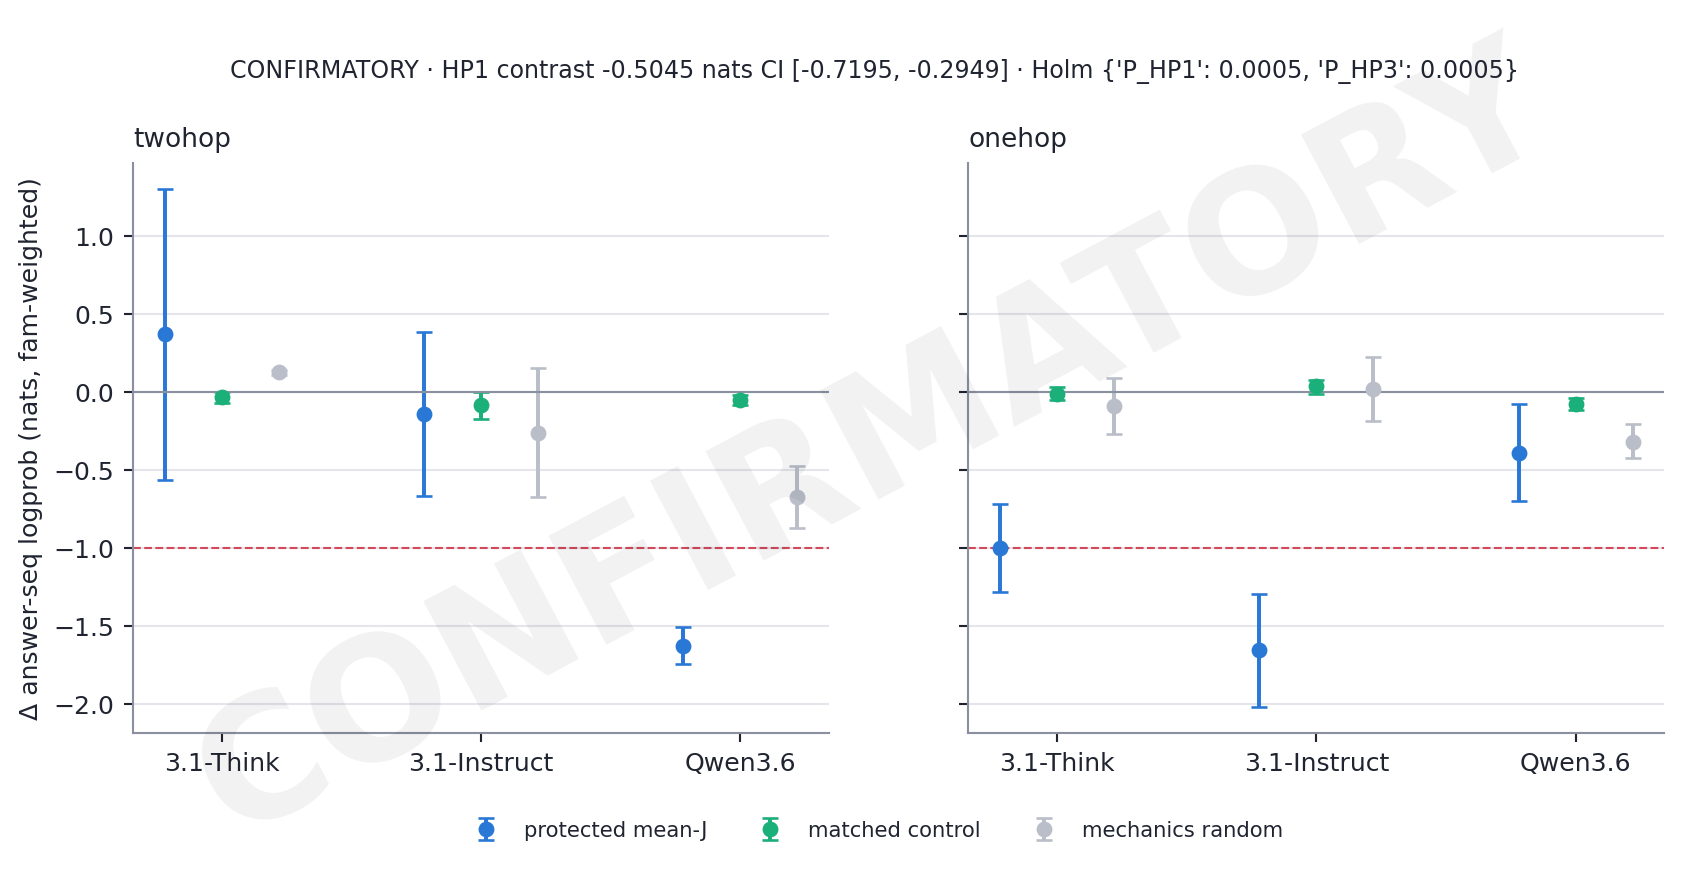
\includegraphics[width=\linewidth]{figures/p2f17_confirmatory_primary.png}
\end{figure}

\textbf{P-HP1 (post-training changes the task contrast): REJECTS}
($p_{\mathrm{holm}}=0.0005$). The Think-vs-Instruct model-by-task
interaction contrast on the logsumexp-alias delta is $-0.504$ nats, CI
$[-0.720, -0.295]$ (172 items, 24 intersection-cohort families,
family-weighted, paired family bootstrap). Transparency note: the
MixedLM formulation agrees in sign ($-0.43$) but cannot represent the
item-level pairing (no crossed random effects in the implementation), so
its interaction test is diffuse ($p=0.71$); the paired family-clustered
bootstrap is the declared fallback and preserves the design. Both are
reported.

\textbf{P-HP3 (a J-specific protected tail beyond geometry): REJECTS on
Qwen} ($p_{\mathrm{holm}}=0.0005$): paired tail-rate difference vs the
geometry-matched control $+0.279$, CI $[+0.205, +0.361]$ ($n=158$
protected-answer items, 32 families), stable across the prespecified
threshold curve ($-0.5$: $+0.32$; $-1.5$: $+0.22$; $-2.0$: $+0.14$) and
under the all-items sensitivity. The OLMo estimates are CI-clean too:
Think $+0.418$ $[0.333, 0.500]$, Instruct $+0.488$ $[0.395, 0.577]$.

\subsection{The matched control did its job}

\code{dyn\_energy\_rank\_matched\_random} --- exact per-position rank and
removed-energy match to the J arm, orthogonal to protected rows ---
produces deltas indistinguishable from zero on every model and task
($-0.08$ to $+0.04$ nats) while the J arm removes nats. At matched dose,
\emph{direction content is the entire effect}. The isotropic
mechanics-random arm meanwhile does real damage on Qwen ($-0.67$
two-hop) at its larger, unmatched dose --- a live illustration of the
dose confound the matched control exists to remove.

\subsection{The shape of the result, and its sharpest caveat}

Qwen's forward dissociation replicates at confirmatory tier (two-hop
$-1.62$ $[-1.74,-1.51]$ vs one-hop $-0.39$); the OLMo 3.1 pair damages
one-hop \emph{more} than two-hop (Think $-1.00$ vs $+0.37$; Instruct
$-1.66$ vs $-0.14$). \textbf{Caveat, stated prominently: the
confirmatory two-hop leg is thin} --- only 9 items / 2 families of the
released two-hop set survived the anchor difficulty window, so the HP1
interaction is carried mostly by the one-hop legs. The untouched
replication partition (32 families) is the built-in check; running it is
the next block's first job.

\subsection{Secondary and guard results}

HP2 (accessibility) is confirmed as an estimate on every model: hard
one-hop items lose $3$--$6\times$ more than easy (Think $-1.80$ vs
$-0.32$; Instruct $-2.67$ vs $-0.85$; Pearson baseline-vs-delta
$+0.37$--$0.41$). The hurdle decomposition puts the one-hop tail rate at
$0.52$--$0.56$ for the OLMo pair with mean magnitude-given-tail $-2.4$
to $-3.3$ nats. The prose-NLL guard shows the protected-J intervention
is not free of nonspecific cost (Instruct $+0.72$ nats prose NLL vs
Think $+0.24$, matched/mechanics controls $\leq 0.16$, logit $\approx
0$) --- worth carrying into interpretation of Instruct's large one-hop
damage.

\subsection{Capacity: the corrected estimand rewrites one pilot headline}

\begin{figure}[h]\centering
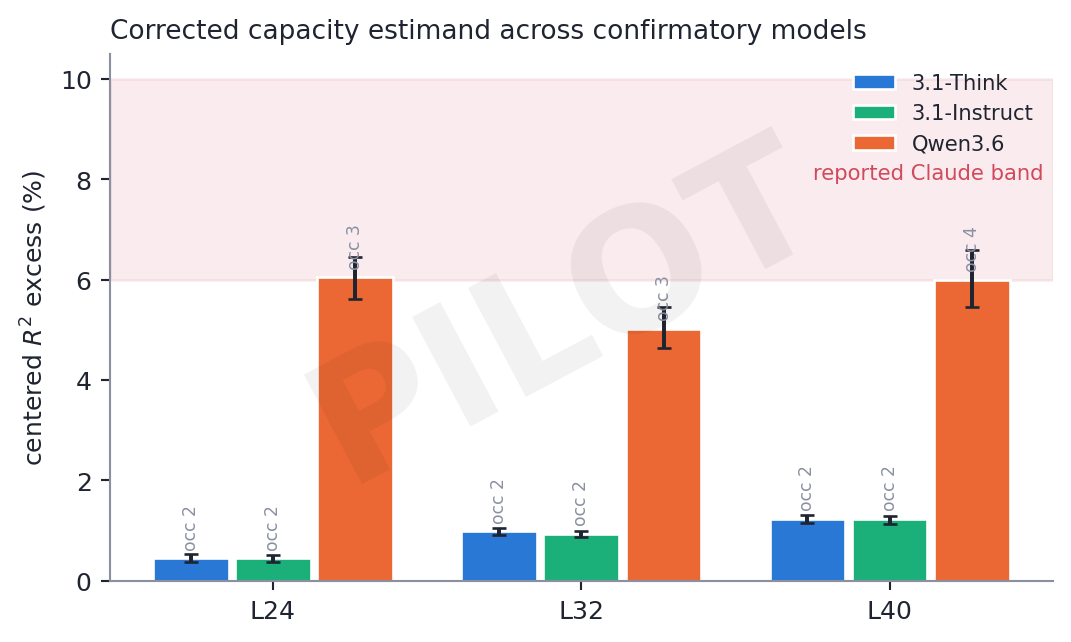
\includegraphics[width=.9\linewidth]{figures/p2f15_capacity_crossmodel.png}
\end{figure}

Own-lens corrected R2 on the primaries: the 3.1 pair are
indistinguishable (occupancy 2.0; centered excess
$0.44/0.98/1.23\%$ vs $0.44/0.94/1.23\%$ at L24/32/40) and replicate the
anchor. \textbf{Qwen lands at $6.05/5.02/5.99\%$ --- the lower edge of
the reported Claude band (6--10\%)}. The pilot's ``all open models an
order of magnitude below Claude'' is withdrawn for Qwen: open-model
capacity spreads $\sim5\times$, and the model with the cleanest causal
dissociation is also the one with near-Claude capacity. (Fit-size
caveat: Qwen's published $n{=}1000$ lens vs OLMo's $n{=}120$ fits ---
prespecified sensitivity.)

\subsection{Instrument notes and amendments (all pre-outcome)}

The \S7 baseline stop rule fired twice before any outcome was viewed and
caught a real two-unit-system inconsistency:
\code{jlens.from\_hf(force\_bos=True)} mutates the shared tokenizer, so
lens fits and all pilot cells live in BOS units while the capability
gate was scored native; and the gate scores answers by piecewise
concatenation of un-rstripped prompts where the pilot grids
string-concatenated. Amendment 1 standardises assay-wide BOS units and
the gate's piecewise convention (capability rescored: Think 774,
Instruct 782, Qwen 875 of 1037; cohorts reassembled as manifest v5,
intersection 700; the frozen partition untouched). The matched-control
dev gate also went through one honest iteration: v1 applied a relative
energy bound below the float32 measurement floor and failed; v2 floors
the relative check at $10^{-3}$ dose with an absolute bound below ---
the same discipline as the withdrawn bf16 linearity v1.

\subsection{Replication partition and the independent-lens clause}

HP3 \textbf{replicates on the 32 held-out families}: Qwen paired
tail-rate $+0.297$ $[+0.207, +0.382]$ vs the confirmatory $+0.279$,
threshold curve stable. HP1 is \emph{inconclusive} on the replication
side (contrast $+0.104$ $[-1.68, +1.89]$, all-items fallback population,
disclosed): the replication two-hop leg is 9 items and absent from the
intersection cohort --- not a contradiction (the CI comfortably contains
the confirmatory $-0.504$), but the thin-two-hop limitation made
concrete. The \textbf{independent-lens clause is fully discharged}: a
second Think lens was fitted on a disjoint corpus (draw B) and both
primaries reproduce their per-item replication deltas almost exactly
under it --- Think $r=0.988$ (tail Jaccard $0.878$), Instruct $r=0.990$
($0.883$). The protected tail is a property of the models, not of any
one lens fit.

\subsection{For further investigation}

(i) Run the replication partition --- especially to thicken the two-hop
leg. (ii) The reverse (one-hop-dominant) OLMo pattern at confirmatory
tier echoes the pilot base-model rung: is one-hop damage the signature
of \emph{rehearsed-fact} channels across the lineage? The HP2 gradient
says accessibility, not hop count, organises the damage. (iii) Qwen's
joint status --- near-Claude capacity, clean forward dissociation, and
the smallest (though CI-clean) matched-control tail gap --- makes the
capacity-vs-causal-shape moderator analysis (prereg's HP4 caution) the
most interesting open thread. (iv) The Instruct prose-guard cost
($+0.72$) deserves a targeted specificity follow-up. (v) The 5/325
trailing-whitespace items carry a double-space tokenization artifact
(cancels in paired deltas; flagged for the mechanism audit).

\section*{Reproducibility}

Run dir \code{special-lab-1/part2\_20260727/} (metrics per model slug,
lenses, logs); code + results mirrored to
\code{interpretability/jspace/part2/} on branch \code{interp\_jspace\_part2};
every figure regenerates from metrics via \code{scripts/p2fig.py}; master
dataset \code{report/matrix\_master.csv}.

\end{document}
